\documentclass[../../../../main.tex]{subfiles}
\begin{document}

\section*{第1問}

\begin{proof}[解]
$0 < p, 0 < q \quad \dots \text{①}$

方程式 $Ap + Bq = 1$ をかんがえる．題意から
\[
  (A, B) = (1, 1), (\cos au, \cos bu), (\cos av, \cos bv)
\]
が解である．よってグラフの概形は右図．$-1 \le A, B \le 1$
だから, $(\cos au, \cos bu), (\cos av, \cos bv) = (1, 1)$ のみ可能．

\begin{center}
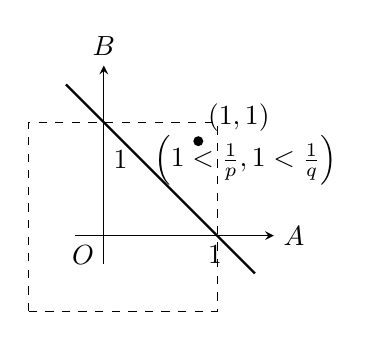
\begin{tikzpicture}[scale=1.2, >=stealth]
  \draw[->] (-0.3,0) -- (1.8,0) node[right] {$A$};
  \draw[->] (0,-0.3) -- (0,1.8) node[above] {$B$};
  \draw[dashed] (-0.8,-0.8) rectangle (1.2,1.2);
  \draw[thick] (-0.4, 1.6) -- (1.6, -0.4);
  \fill (1,1) circle (1.5pt);
  \node[above right] at (1,1) {$(1,1)$};
  \node[below left] at (0,0) {$O$};
  \node[below right] at (0,1) {$1$};
  \node[below right] at (1,0) {$1$};
  \node at (1.5, 0.8) {$\left(1 < \frac{1}{p}, 1 < \frac{1}{q}\right)$};
\end{tikzpicture}
\end{center}

したがって，
\[
  \begin{cases}
    \cos au = \cos av = 1 \\
    \cos bu = \cos bv = 1
  \end{cases}
\]
だから，整数 $k_1 \sim k_4$ を用いて
\[
  \begin{cases}
    au = 2k_1 \pi, & bu = 2k_2 \pi \\
    av = 2k_3 \pi, & bv = 2k_4 \pi
  \end{cases}
\]
となる．$a \neq 0$ の時，$u = \dfrac{2k_1 \pi}{a}, v = \dfrac{2k_3 \pi}{a}$ から $\dfrac{v}{u} = \dfrac{k_3}{k_1} \in \mathbb{Q}$ となり矛盾するから，$a = 0$．

同様に $b = 0$ だから，題意は示された．
\end{proof}

\newpage

\section*{第2問}

\begin{proof}[解]
$f(0) = 1, f\left(\dfrac{\pi}{2}\right) = 1$ から，
\[
  \begin{cases}
    1 = a + b \\
    1 = a + c
  \end{cases}
  \quad \therefore b = c = 1 - a \quad \dots \text{①}
\]
である．したがって，
\begin{align*}
  f(x) &= a + (1-a)(\cos x + \sin x) \\
  f'(x) &= (1-a)(\cos x - \sin x) \\
  &= \sqrt{2}(1-a)\cos\left(x + \frac{\pi}{4}\right) \quad \dots \text{②}
\end{align*}
だから，$a$ によって下表をえる．

\paragraph{$1^\circ$ $1-a < 0 \quad \therefore 1 < a$ の時}

\begin{center}
\begin{tabular}{c|ccccc}
$x$ & $0$ & $\dots$ & $\pi/4$ & $\dots$ & $\pi/2$ \\ \hline
$f'$ & & $-$ & $0$ & $+$ & \\ \hline
$f$ & $1$ & $\searrow$ & & $\nearrow$ & $1$
\end{tabular}
\end{center}

したがって，$|f(x)| \le 2$ となる条件は
\[
  f\left(\frac{\pi}{4}\right) \ge -2 \iff a \le \sqrt{2}
\]

\paragraph{$2^\circ$ $1-a = 0 \quad \therefore a = 1$ の時}
$f(x) \equiv 1$ から，条件を満たす．

\paragraph{$3^\circ$ $1-a > 0 \quad \therefore a < 1$ の時}

\begin{center}
\begin{tabular}{c|ccccc}
$x$ & $0$ & $\dots$ & $\pi/4$ & $\dots$ & $\pi/2$ \\ \hline
$f'$ & & $+$ & $0$ & $-$ & \\ \hline
$f$ & $1$ & $\nearrow$ & & $\searrow$ & $1$
\end{tabular}
\end{center}

条件は
\[
  f\left(\frac{\pi}{4}\right) \le 2 \iff -\sqrt{2} \le a
\]

以上から，$ -\sqrt{2} \le a \le \sqrt{2}$．
\end{proof}

\newpage

\section*{第3問}

\begin{proof}[解]
$c = \cos\theta, s = \sin\theta$ とおく ($0 \le \theta < 2\pi$)．題意から $(x,y) = (c,s)$ とおける．

$f(\theta) = x^2 - y^2 + 2\sqrt{3}xy$ とすると
\[
  f(\theta) = \cos 2\theta + \sqrt{3}\sin 2\theta = 2\sin\left(2\theta + \frac{\pi}{6}\right)
\]
だから $f(\theta)$ が最大の時，$\theta = \dfrac{\pi}{6}, \dfrac{7}{6}\pi$ で $(x,y) = \left(\dfrac{\sqrt{3}}{2}, \dfrac{1}{2}\right), \left(-\dfrac{\sqrt{3}}{2}, -\dfrac{1}{2}\right)$．

$f(\theta)$ が最小の時，$\theta = \dfrac{2}{3}\pi, \dfrac{5}{3}\pi$ で $(x,y) = \left(-\dfrac{1}{2}, \dfrac{\sqrt{3}}{2}\right), \left(\dfrac{1}{2}, -\dfrac{\sqrt{3}}{2}\right)$．
\end{proof}

\newpage

\section*{第4問}

\begin{proof}[解]
$A(1,0), B(-1,0), C(t,0)$ ($0 \le t \le 1$) とおく．

対称性から，$P, Q$ の $y$ 座標が正である時のみをかんがえる．この時，題意の2円は
\[
  \begin{cases}
    \left(x - \dfrac{1+t}{2}\right)^2 + y^2 = \left(\dfrac{1-t}{2}\right)^2 \\[8pt]
    \left(x - \dfrac{-1+t}{2}\right)^2 + y^2 = \left(\dfrac{1+t}{2}\right)^2
  \end{cases}
  \quad \dots \text{①}
\]
図のように角度 $\theta$ をおくと，接線は，$c = \cos\theta, s = \sin\theta$ とおくと
\[
  \begin{cases}
    c\left(x - \dfrac{1+t}{2}\right) + sy = \dfrac{1-t}{2} \\[8pt]
    c\left(x - \dfrac{-1+t}{2}\right) + sy = \dfrac{1+t}{2}
  \end{cases}
\]
これらが等しい時
\[
  c \frac{1+t}{2} + \frac{1-t}{2} = c \frac{-1+t}{2} + \frac{1+t}{2}
\]
\[
  \therefore c = t
\]
だから $s = \sqrt{1-t^2}$ で
\begin{align*}
  P\left(\frac{1+t}{2} \cdot t + \frac{1-t}{2}, \frac{1-t}{2}\sqrt{1-t^2}\right) \\
  Q\left(\frac{1-t}{2} \cdot t + \frac{1+t}{2}, \frac{1+t}{2}\sqrt{1-t^2}\right)
\end{align*}
だから，$PQ$ の中点 $M(X,Y)$ とすると
\[
  \begin{cases}
    X = \dfrac{1}{2}\left\{\dfrac{t^2+2t-1}{2} + \dfrac{-t^2+2t+1}{2}\right\} = t \\[8pt]
    Y = \dfrac{1}{2}\left\{\dfrac{1+t}{2} + \dfrac{1-t}{2}\right\}\sqrt{1-t^2} = \dfrac{1}{2}\sqrt{1-t^2} = \dfrac{1}{2}\sqrt{1-X^2}
  \end{cases}
\]
したがって，対称性から，$X^2 + 4Y^2 = 1$ が求める軌跡である．

\begin{center}
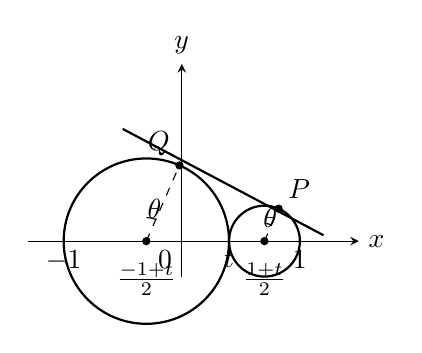
\begin{tikzpicture}[scale=1.5, >=stealth]
  \draw[->] (-1.3,0) -- (1.5,0) node[right] {$x$};
  \draw[->] (0,-0.3) -- (0,1.5) node[above] {$y$};
  
  \draw[thick] (-0.3,0) circle (0.7);
  \draw[thick] (0.7,0) circle (0.3);
  
  \fill (-0.3,0) circle (1pt);
  \fill (0.7,0) circle (1pt);
  
  \draw[thick] (-0.5, 0.95) -- (1.2, 0.05);
  
  \fill (-0.02, 0.641) circle (1pt) node[above left] {$Q$};
  \fill (0.82, 0.275) circle (1pt) node[above right] {$P$};
  
  \draw[dashed] (-0.3,0) -- (-0.02, 0.641);
  \draw[dashed] (0.7,0) -- (0.82, 0.275);
  
  \node[below] at (-1,0) {$-1$};
  \node[below] at (-0.3,-0.1) {$\frac{-1+t}{2}$};
  \node[below left] at (0,0) {$0$};
  \node[below] at (0.4,0) {$t$};
  \node[below] at (0.7,-0.1) {$\frac{1+t}{2}$};
  \node[below] at (1,0) {$1$};
  
  \draw (-0.3,0.2) arc (90:66:0.2);
  \node at (-0.23,0.27) {$\theta$};
  
  \draw (0.7,0.15) arc (90:66:0.15);
  \node at (0.75,0.2) {$\theta$};
\end{tikzpicture}
\end{center}
\end{proof}

\newpage

\section*{第5問}

\begin{proof}[解]
$F(x) = \int_0^x f(t) dt$ とおく．$F(x) = \dfrac{1}{4}x^4 + \dfrac{p}{3}x^3 + \dfrac{q}{2}x^2 + rx$ である．

\[
  (\text{与式}) \iff 2F(x) \le F(x+y) + F(x-y)
\]
だから代入して
\begin{align*}
  \frac{1}{4}\left[(x+y)^4 + (x-y)^4 - 2x^4\right] + \frac{p}{3}\left[(x+y)^3 + (x-y)^3 - 2x^3\right] \\
  + \frac{q}{2}\left[(x+y)^2 + (x-y)^2 - 2x^2\right] + r\left[(x+y) + (x-y) - 2x\right] &\ge 0 \\[5pt]
  \frac{1}{4}\left[12x^2 y^2 + 2y^4\right] + \frac{p}{3}\left[6xy^2\right] + \frac{q}{2}\left[2y^2\right] &\ge 0 \\[5pt]
  3x^2 + \frac{1}{2}y^2 + \frac{1}{3}px + q &\ge 0 \quad (\because y^2 \ge 0)
\end{align*}
だから，$3x^2 + \dfrac{p}{3}x + q = 0$ の判別式 $D$ として，条件式は
\[
  D \le 0 \iff \left(\frac{p}{3}\right)^2 - 12q \le 0 \iff p^2 \le 108q
\]
\end{proof}

\newpage

\section*{第6問}

\begin{proof}[解]
$-\dfrac{1}{2} < f'(x) < \dfrac{1}{2} \quad \dots \text{①}$ の両辺 積分して，$-\dfrac{1}{2}x + C_1 < f(x) < \dfrac{1}{2}x + C_2$ である． $\dots \text{②}$

\begin{enumerate}[(1)]
  \item $F(x) = f(x) - x$ とおく．$F'(x) = f'(x) - 1 < 0$ から，$F(x)$ は単調減少で，②から
  \[
    -\frac{3}{2}x + C_1 < F(x) < -\frac{1}{2}x + C_2
  \]
  だから，はさみうちから，$x \to \infty$ で $F(x) \to -\infty$，$x \to -\infty$ で $F(x) \to +\infty$ であり，$F(x)$ は連続だから，以上から $F(x) = 0$ はただ1つの実解を持つ．

  \item $f(\alpha) = \alpha$ から，
  \[
    a_{n+1} - \alpha = f(a_n) - f(\alpha) \quad \dots \text{③}
  \]
  $a_m = \alpha$ なる $m$ がある時，③から，$n \ge m$ をみたす $n$ に対して，$a_n = \alpha$ だから，$a_n \to \alpha \ (n \to \infty)$ である．

  その他の時，平均値の定理から，$f(a_n) - f(\alpha) = f'(c)(a_n - \alpha)$ をみたす $c$ がある．③から
  \[
    |a_{n+1} - \alpha| = |f'(c)||a_n - \alpha| < \frac{1}{2}|a_n - \alpha| \quad (\because \text{①})
  \]
  くり返し用いて，
  \[
    |a_n - \alpha| < \left(\frac{1}{2}\right)^{n-1}|a_1 - \alpha| \xrightarrow{n \to \infty} 0
  \]
  はさみうちから，
  \[
    a_n \longrightarrow \alpha \quad (n \to \infty)
  \]
\end{enumerate}
\end{proof}

\end{document}
